%\documentclass[Japanese]{dicomopapers}
\documentclass[Japanese,noauthor]{dicomopapers}

\usepackage[dvipdfmx]{graphicx}
\usepackage{latexsym}
\usepackage{bm}
%\usepackage{comment}

\def\Underline{\setbox0\hbox\bgroup\let\\\endUnderline}
\def\endUnderline{\vphantom{y}\egroup\smash{\underline{\box0}}\\}
\def\|{\verb|}

\def\newblock{\hskip .11em plus .33em minus .07em}

\begin{document}

% 和文表題
\title{圧力センサ搭載ヘルメットを用いた\\個人識別手法の提案}

% 所属ラベルの定義
\affiliate{RU}{立命館大学 情報理工学部}
\affiliate{JST}{JSTさきがけ}

\author{藤井 敦寛}{ATSUHIRO FUJII}{RU}
\author{村尾 和哉}{KAZUYA MURAO}{RU, JST}

\begin{abstract}
ヘルメットは社会生活において広く利用されている.例えば,野球やアメリカンフットボールなどのスポーツ用や二輪車用のヘルメットが存在する.また,工事現場では作業者は頭部を保護するためにヘルメットを装着することが一般的であり,視線情報を記録可能なウェアラブルカメラを取り付けたヘルメットが販売されている.さらに,通信機能をもつ防災用ヘルメット\cite{disaster}が提案されている.このように,さまざまな機能をもつヘルメットがある.本研究では圧力センサを搭載したヘルメットを装着することで,頭部形状から個人を識別する手法を提案する.提案手法によって,ヘルメット上部に取り付けたディスプレイに名前を表示したり,視線情報などのセンサデータを取得する際に作業者のラベルを付与できる.また,工場などで役職により入室できる部屋が制限されている場合に扉の鍵として使用できる他,二輪車の鍵としても用いることができる.鍵として用いる場合,ヘルメットでの本人識別を挟むため,鍵の盗難による侵入,車両盗難のリスク回避にも繋がる.認証には様々な手法が存在するが,現在広く用いられている指紋認証\cite{finger_print}や顔認証\cite{face}などは,ヘルメットが工場や屋外などの厳しい条件下で着用され,汚れや水没の可能性があることを考慮するとあまり適さない.また,ヘルメットに実装する場合,デバイスが軽量かつ視界を遮らないという条件を満たさなければならない.これらの条件を考慮し,本研究では圧力センサを搭載したヘルメットを装着することで個人識別を行う手法を提案する.識別には特徴があり複製が難しいものとして頭部形状を使用した.また,頭部状態の測定にヘルメットを用いている先行研究は筆者らの知る限りは存在しない.そのため,提案手法は頭部装着型デバイスとしての新規性がある.提案手法は,ヘルメットに搭載した32個の圧力センサから得られたセンサ値をベクトルとして扱い,事前に登録フェーズで蓄積しておいた所有者のセンサデータ群とのマハラノビス距離を計算し,閾値を用いて識別を行う.本手法で用いるデバイス,およびソフトウェアを設計,実装し評価実験を行った.プロトタイプデバイスは市販のフルフェイス型のヘルメットを加工し圧力センサを取り付け,マイコンに配線することで実装した.解析用のソフトウェアはPythonのscikit-learnのsklearn.covariance.MinCovDetを使用してマハラノビス距離を計算し,閾値を移動しながら評価指標であるFRR,FAR,EERを求めるよう設計した.ソフトウェアを実装した後,評価用に被験者9人からそれぞれ2秒間のセンサ値を20回分収集した.これらのデータセットからマハラノビス距離を用いて識別を行う.5分割交差検証を行い,被験者全員の平均EERが約7.8\%という結果が得られた.
\end{abstract}

% 表題などの出力
\maketitle

% 本文はここから始まる
\section{はじめに}
\label{introduction}
現在販売されている四輪車の多くにスマートキーシステムが導入されている.スマートキーシステムとは,キーをポケットなどに入れて接近するとキーから発せられる電波を車が感知してドアの解錠を行い,離れるとドアの施錠を行う機能である.キーを持ったままボタンを押すだけでエンジンを始動することもできる.スマートキーシステムは二輪車にも導入されつつある.二輪車におけるスマートキーシステムも四輪車と同様に,キーを所持しておくだけでキーシリンダーにキーを挿し込む手間なく,ラゲッジスペースと呼ばれる荷物を収納するスペースの解錠やエンジンの始動を可能にする機能である.しかしながら,スマートキーシステムはキーを所持しておかなければならず,キーの紛失や第三者がキーを入手することで車両盗難のリスクがある.\par

物理的な鍵以外で本人を認証する手法として,パスワードなどの知識や筆跡などの行動的特徴,指紋などの身体的特徴を用いる手法がある.当麻ら\cite{face}はステレオカメラを用いた顔認証システムを提案しており,ヘルメット装着前に二輪車に取り付けられたカメラの方を向くことで実現可能であると考えられる.しかし,カメラの電源を入れてカメラの方を向く必要があり,二輪車を運転するたびにこのような操作を行うのは面倒である.また,本人の写真やお面で認証を破ることができるリスクもある.このほか,指紋認証のアプローチもあるが,指紋は写真などから簡単に複製されるリスク\cite{finger_print}がある.\par

本研究では,二輪車での走行において法令で装着が義務付けられているヘルメットに着目し,ヘルメットを用いた本人認証が実現できれば,既存のキーを用いたシステムの問題点を解決できると考え,搭乗者が圧力センサを搭載したヘルメットを装着することで,搭乗者の頭部形状にもとづき本人認証をする手法を提案する.頭部形状は個人ごとに異なり,頭部形状の取得や複製は困難であると考える.具体的には,あらかじめ車両とペアリングして所有者の頭部形状データを登録しておいたヘルメットを二輪車のヘルメットロックに装備しておく.ヘルメットロックに繋がったまま利用者がヘルメットを装着し,取得した頭部形状と事前に登録した頭部形状が一致すればロックが外れ,エンジンを始動できるようになるという想定である.\par

提案手法によって利用者は何も持たずに乗車できるため,キーの紛失や盗難のリスクを減少させることができる.一方で,登録された利用者以外がヘルメットをかぶった場合は本人として認証されず,ヘルメットロックも外れず,エンジンの始動もできないため,車両盗難のリスクも減少させることができる.\par

以降本稿では,\ref{related}章で関連研究を紹介する.\ref{method}章で提案手法を説明し,\ref{make}章で実装について述べる.\ref{evaluation}章で提案手法の評価実験と結果の考察を行い,最後に\ref{conclude}章で本研究をまとめる.

\section{関連研究}
\label{related}
本章では個人認証手法,頭部装着型デバイス,頭部状態認識に関する研究を紹介する.
\section{個人認証手法}
%車両にカメラを取り付ける手法
当麻ら\cite{face}はステレオカメラを用いた顔認証システムを提案している.既存の顔認証システムではカメラに意識して顔を向ける必要があった.その問題を解決するため,少数の正面を向いていない顔画像から正面顔画像を作成し,個人認証を行う手法を提案している.佐藤ら\cite{door}は掌紋認証を装備したインテリジェントドアノブシステムの開発をしている.このシステムでは,認証に特別な動作を必要とする煩わしさを解決するため,ドアノブにカメラを装着し掌紋の画像を取得する.得られた画像からSIFT特徴を用いて認証を行う.

%ヘルメットでのジェスチャー認証
成ケ澤ら\cite{acceleration}はスマートフォン内蔵の加速度センサとジャイロセンサを用い,ユーザがスマートフォンを手のひらの上で回転させる動作を行うことで,その加速度と角速度の特徴量から認証する手法を提案している.

%ヘルメットに搭載可能な別認証手法
白川ら\cite{iris_eye}は虹彩と目の周辺画像を統合して認証する手法を提案している.虹彩認証は高画質の画像を必要とし,至近距離で認証を行う必要があり,被認証者に負担を与えてしまう.そこで目頭や目尻,まぶたの形などに個人差が存在することに注目し,目の周辺の分割画像を利用して目の周辺認証を行い,虹彩と統合する認証を提案した.岸里ら\cite{mouth_pattern}は口唇領域の動きの画像認識を用いたスマートデバイス向けパターンロックシステムを提案している.スマートフォンやタブレット端末のパターンロック認証は,肩越しに画面を覗き見るショルダーハックや,画面に残った脂の跡を読み取ることによって,認証キーを盗まれてしまうリスクをもつ.そこで手の指の代わりに,端末のカメラで口唇領域の動きを認識し,画面に触れることなく認証を行うシステムを提案した.越前ら\cite{finger_print}は写真からの指紋復元の脅威とその対策技術を提案している.指紋認証には複製の恐れがあり,少ない写真でも簡易に複製が可能である.そのため,指にジャミングパターンを装着する対策技術を提案した.

%上記の認証手法へのダメ出しと提案手法の強み
これらは個人認証の手法であり,いずれも二輪車のキーとして応用ができる可能性がある.顔認証を行う場合,カメラをあらかじめ車両に取り付けておき,ヘルメットを装着する前にカメラの方を向くことでシステムを実装することが可能である.掌紋画像での認証の場合は二輪車のハンドルにカメラを取り付けることで実装可能である.しかし,どちらの手法も悪天候による水没,走行時の衝撃からの耐久性を考慮しなければならない.また,認証時にカメラの電源を入れる手間が生じる.したがって,カメラを車両に取り付ける必要のある手法は向かない.ジェスチャ認証の場合,ヘルメットに加速度センサとジャイロセンサを搭載することで,ヘルメットを被るまでの動作の加速度と角速度の特徴量を用いて認証できる可能性がある.しかしながら,急いでいて動作が速くなる場合や,雨天時にヘルメットの内装が濡れないように気をつけながら装着する場合など,ヘルメットを装着する動作が変化する可能性が考えられる.状況の変化を考慮すると,ヘルメットを静止させたまま認証が可能な手法が適切である.

目を用いた認証手法の場合,ヘルメットを動かすことなく認証が可能である.しかし,虹彩や目の周辺の分割画像を取得するには目の前付近にカメラを設置する必要がある.そのため,ヘルメットに実装する場合,視界を遮る恐れがある.口唇領域の画像であれば視界を遮らずに撮影できるが,ヘルメットの口元の空間は限られる.そのため,口とカメラの距離が近くなってしまい,1個のカメラで口唇領域の動きを判別することは難しくなる.カメラの数を増やすとヘルメットの重量増加に繋がる.

そこで,本研究では内装に圧力センサを搭載したヘルメットを装着することで,頭部形状を取得して個人認証する手法を提案する.提案手法は個人認証のために特別な動作を必要とせず,デバイスの搭載によって視界を遮ることもない.さらに,認証に用いる頭部形状を複製するには立体形状を正確に把握する必要があり,複製が困難である.

\section{頭部装着型デバイス}
%デバイスとしての新規性
田中ら\cite{glasses}はメガネ型デバイスを用いた経皮水分蒸散量の常時測定システムを提案している.皮膚状態の診断には経皮水分蒸散量などの定量的な指標が用いられるが,測定には高価な機器が必要で,また定常的な測定はできない.そこで,定常的に測定を行い皮膚の健康維持を支援するため,メガネ型デバイスに2つの温度・湿度センサを装着し,皮膚状態の評価指標である経皮水分蒸散量の常時測定を行うシステムを提案した.石井ら\cite{happymouth}は人間の対面コミュニケーション能力を拡張するマスク型デバイス「HappyMouth」を提案している.このシステムでは,マスクに小型ディスプレイが内蔵されており,口元の映像を提示できる.映像提示の機能として,ユーザが自分の好みの口を選択して表示する機能,ユーザの発話をテキスト化して字幕表示する機能,ユーザの発したキーワードをインターネットで画像検索した結果を表示する機能がある.新島ら\cite{cap_sensor}は左右の側頭筋の筋活動を測定することができる,導電性高分子の布電極を用いた帽子型筋電センサhitoeCapを提案している.これは食事や睡眠や運動などの日々の生活の様々な場面で活動する,咀嚼筋の一つである側頭筋の筋電データを測定すれば,ユーザのライフログとして活用できると考え提案された.これらの研究はいずれも頭部に装着するデバイスであり,様々な形状のデバイスが提案されている.しかしながら,頭部装着型デバイスとしてヘルメットを用いた研究は筆者の知る限り存在しない.

\section{頭部状態の認識}
%頭部形状を認識するという点での新規性
近年注目されているヒアラブルデバイスにおいて求められる機能のひとつとして,手や視界を占有することのないデバイス操作機能が挙げられる.既存の製品や既存の研究では認識精度や認識できるジェスチャの種類,頑健性などの点で課題が残る.これらの課題を解決するために雨坂ら\cite{ear}は首,顎,顔の状態(頭部状態)にともなって外耳道が変形することに着目し,外耳道インパルス応答を測定することで頭部状態を認識する手法を提案した.一方,状況の変化に関して口周辺の動作に着目すると,感情や咀嚼といった様々な情報が含まれており,これらを認識することで感情の記録や,咀嚼カウントによる肥満防止など,新たなコンテキストアウェアサービスが提供できる.そこで,山下ら\cite{mouth}は日常生活での利用を想定し,安価な付け髭型デバイスを用いた口周辺の形状変化によるコンテキスト認識手法を提案した.これらの研究は表情や動作などの動的な情報を取得するものであり,対して本研究は静的な頭部形状そのものの特徴を取得するという点で異なる.

\section{提案手法}
\label{method}
本章では提案手法の詳細を述べる.

認識対象の装着者はヘルメットを被った状態で2ms 静
止し,その間のセンサデータを蓄積する.このデータは32
個の圧力センサの電圧値を要素とする32 次元のベクトル
であるが,識別に必要なデータは1 回被った時に1 ベクト
ルのみであるため,この2ms のデータの平均値を用いる
こととする.これらのサンプルを用いて,登録者のうち誰
が装着したのかを判別することを目的とした教師あり学習
と,二輪車の鍵として用いることを想定し,持ち主である
か他人であるかを判別する教師なし学習を行う.教師あり
学習ではSupport Vector Machine を用いて32 次元のベク
トルの特徴を解析する.一方で,教師なし学習では持ち主
と仮定した被験者のデータ群と入力データのマハラノビス
距離を計算し,閾値を用いて判別する.

\section{概要}
本研究はヘルメットをキーの代わりとして用いることを目標とし,利用者が圧力センサを搭載したヘルメットを装着して,頭部形状を取得することで,本人認証を行う手法を提案する.提案するシステムの構成を図\ref{system}に示す.ヘルメットの内側には32個の圧力センサが搭載されており,1回のサンプリングで32次元のデータを取得する.提案するシステムでは,あらかじめ学習フェーズとして,二輪車の所有者など認証したいユーザの頭部の32次元の圧力センサデータを,ヘルメットを複数回装着することで収集しておく.そして,識別フェーズでは,ヘルメットを装着した人物の32次元の圧力センサデータと事前に収集した学習データの距離を計算し,距離が閾値以下であれば本人であると認証する.

\section{登録データとの距離計算}
学習データと入力データの距離計算方法として,マハラノビス距離を用いる.マハラノビス距離とは多変数間の距離計算手法のひとつであり,データの分布を考慮して正規化した距離を計算できる.学習データを$\bm{x}_i~(i=1,\dots, m)$,認証するユーザの入力データを$\bm{y}$とする.ただし,$m$は学習データの個数である.
学習データの平均値ベクトル$\bm{\mu}$と分散共分散行列$\bm{\Sigma}$を次式で求める.
\begin{eqnarray}
  \bm{\mu} &=& \frac{1}{m}\sum_{i=1}^{m}\bm{x}_i \\
  \bm{\Sigma} &=& \frac{1}{m}\sum_{i=1}^{m}(\bm{x}_i-\bm{\mu})(\bm{x}_i-\bm{\mu})^T
\end{eqnarray}
このとき,入力データが事前に登録された本人のデータであれば,学習データ$\bm{x}_i$と入力データ$\bm{y}$は同じ分散共分散行列$\bm{\Sigma}$の確率分布に従うため,学習データ$\bm{x}_i$と入力データ$\bm{y}$のマハラノビス距離は
\begin{eqnarray}
  d(\bm{y},\bm{x}_i) = \sqrt{(\bm{y}-\bm{x}_i)^{T}\bm{\Sigma}^{-1}(\bm{y}-\bm{x}_i)}
\end{eqnarray}
と定義できる.

\section{認証判定}
閾値を$\theta$とおき,
\[
  \theta < min_i(d(\bm{y},\bm{x}_i))~(i=1,\dots,m)
\]
を満たす場合,入力データ$\bm{y}$は所有者以外の他人から得られた頭部データであると判定し拒否する.
一方で,
\[
  \theta \geq min_i(d(\bm{y},\bm{x}_i))~(i=1,\dots,m)
\]
を満たす場合,入力データ$\bm{y}$は所有者本人から得られた頭部データであると判定し認証する.

\begin{figure}[!t]
  \centering
    \includegraphics[width=1\linewidth]{figure/system.eps}
  \caption{システム構成}
  \label{system}
\end{figure}

\section{実装}
\label{make}
本章では実装したヘルメットのハードウェアとソフトウェアを説明する.

\section{ハードウェア}
提案手法に用いる圧力センサを搭載したヘルメットを実装した.デバイスの構成を図\ref{device},プロトタイプデバイスの写真を図\ref{met_over}に示す.

圧力値を正しく取得するには,センサとヘルメット装着者の頭部が密着している必要があるため,フルフェイス型ヘルメット(B\&B社製BB100)を用いた.圧力センサとしてインターリンクエレクトロニクス社製のFSR402およびFSR402 ShortTailを合計32個使用した.
マイコンとしてArduino MEGA2560 R3を使用した.

実装したプロトタイプデバイスの内部を図\ref{met_in}に示す.今回用いたヘルメットはフリーサイズであり,また内装の脱着が困難であったため,頭頂部の内装を取り外して,新たに厚みのあるウレタンスポンジを取り付けた.図\ref{sensor}のようにウレタンスポンジの中央部に切り込みを入れて圧力センサを挿し込んだ.圧力センサは頭頂部に4個,頭頂部周囲に16個,後頭部に6個,左右チークパッド部に6個の合計32個を搭載した.配線はヘルメットの頭頂部にドリルで開けた穴から,ヘルメット外部に取り付けた10KΩの抵抗を配線してあるプリント基板を経由して,Arduino MEGA2560 R3の5V電源,GND,アナログ入力ポートに接続した.このプリント基板を図\ref{print}に示す.プリント基板は取り外しが可能なように,ヘルメットのシールド固定用に開けられたネジ穴を用いて左頬部分にボルトで固定している.

\begin{figure}[!t]
  \begin{center}
    \includegraphics[width=0.65\linewidth]{figure/device.eps}
  \end{center}
  \caption{デバイス構成}
  \label{device}
\end{figure}

\begin{figure}[!t]
  \begin{center}
    \includegraphics[width=0.6\linewidth]{figure/met_over.eps}
  \end{center}
  \caption{プロトタイプデバイスの全体図}
  \label{met_over}
\end{figure}

\begin{figure}[!t]
  \begin{center}
    \includegraphics[width=0.6\linewidth]{figure/met_in.eps}
  \end{center}
  \caption{プロトタイプデバイスの内部}
  \label{met_in}
\end{figure}

\begin{figure}[!t]
  \begin{center}
    \includegraphics[width=0.6\linewidth]{figure/sensor.eps}
  \end{center}
  \caption{センサの実装方法}
  \label{sensor}
\end{figure}

\begin{figure}[!t]
  \begin{center}
    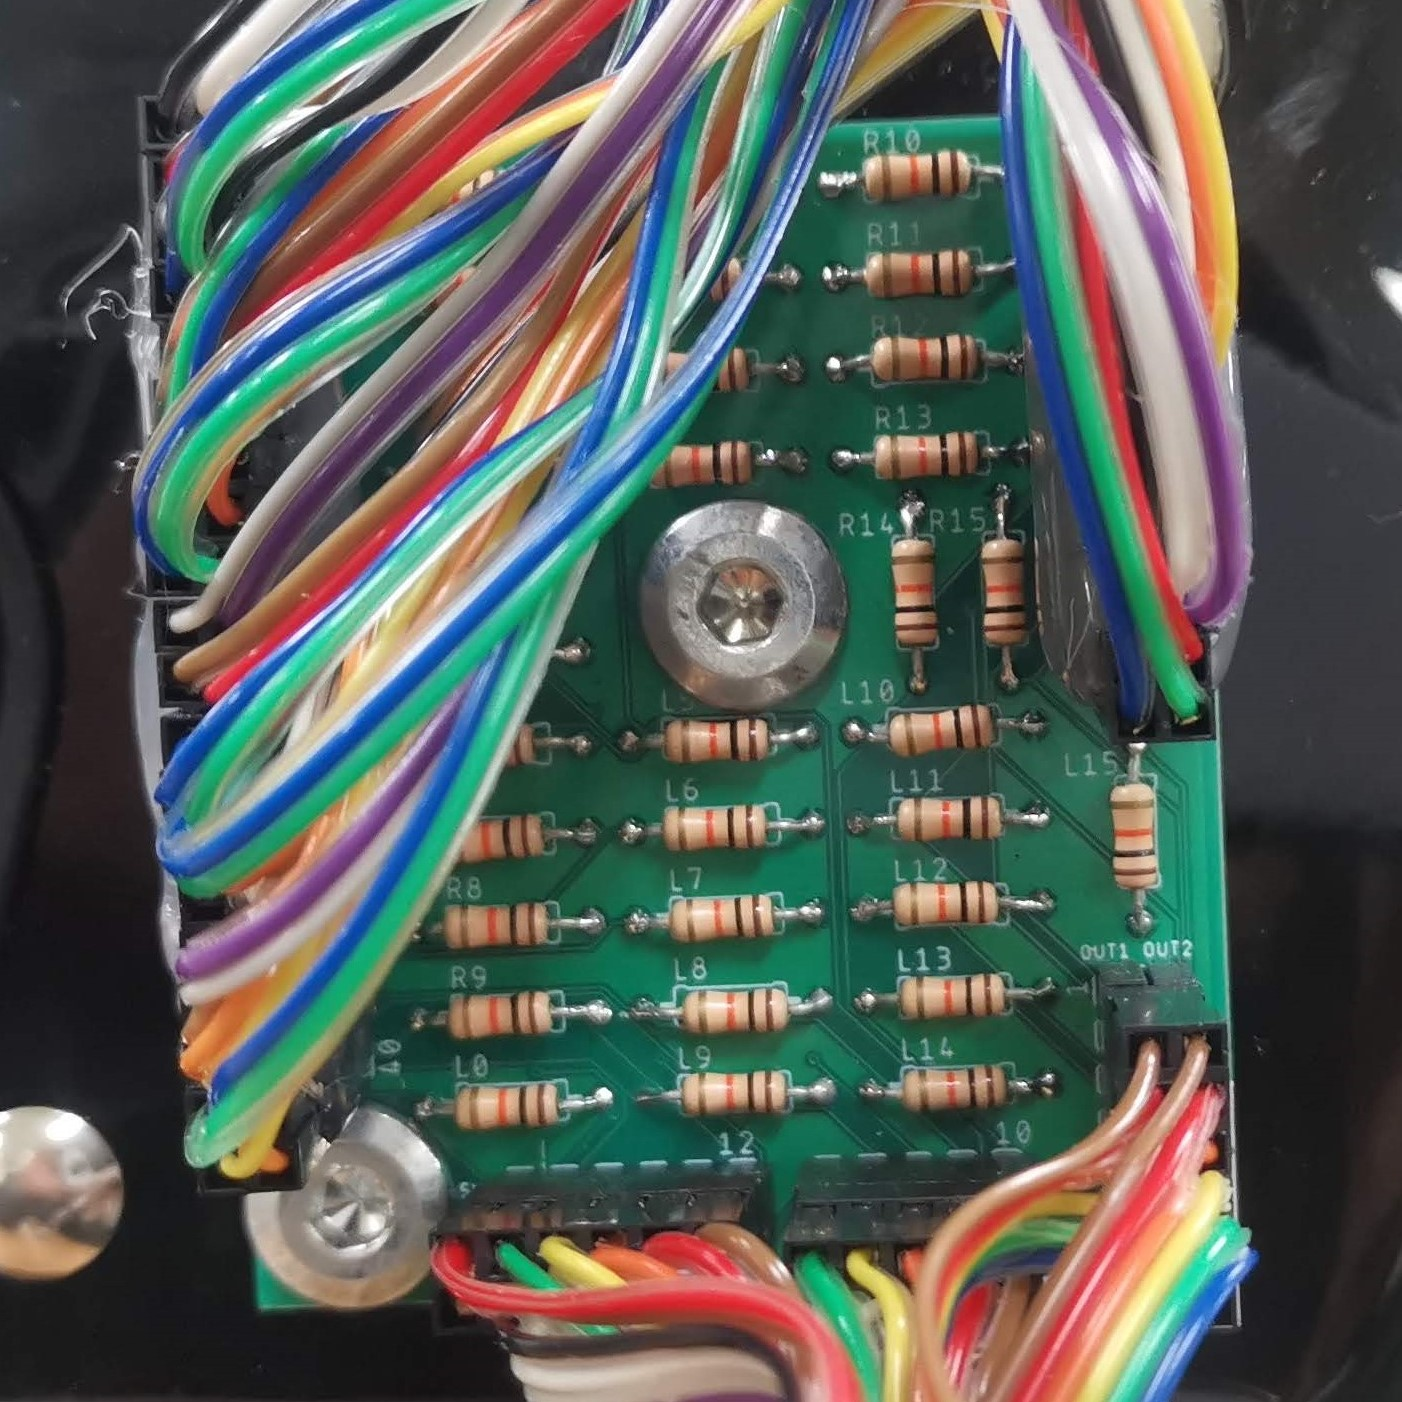
\includegraphics[width=0.6\linewidth]{figure/print.eps}
  \end{center}
  \caption{プリント基板}
  \label{print}
\end{figure}

\section{ソフトウェア}
Arduino MEGAのプログラムはArduinoIDEで実装した.マイコンからコンピュータへのデータの受信はPythonで実装し,センサデータをコンピュータ上にcsv形式で保存する.
データの解析はPythonで実装し,事前に収集したセンサデータのcsvファイルを読み出し,sklearn.covariance.MinCovDetを用いて分散共分散行列を計算する.その分散共分散行列の逆行列から,scipy.spatial.distanceを用いて学習データ$\bm{x}_i$のすべてに対する入力データ$\bm{y}$のマハラノビス距離を計算する.
sklearn.covariance.MinCovDetとは,異常値に対して頑健な分散共分散行列の推定アルゴリズムであるMinimum Covariance Determinant (MCD)を高速化したFast-MCD\cite{fast_mcd}を実装したscikit-learnのライブラリである.また,scipy.spatial.distanceとは,様々な距離計算の関数を実装したSciPyのライブラリである.

\section{評価}
\label{evaluation}
本章では,提案手法の有効性を評価するために行った実験について説明する.

\section{データ収集}
被験者9名(A$\sim$I,全員男性,平均年齢23歳)に実装したヘルメットを装着させ,サンプリングレート約30Hzでセンサデータを収集した.2秒間装着して取り外し再び2秒装着する試行を1セットとして被験者1人あたり10セット,合計20回装着するデータ(2秒$\times$2回$\times$10セット)を収集した.データの収集は1人当たり1日最大4セットとし,複数日に渡ってデータを収集した.センサと頭部のさまざまな位置関係のデータを収集するために,セット間に30分以上の休憩時間を設けた.1回2秒間32次元の装着データの時間平均値を算出し,1回の装着から32次元のベクトルを1サンプル得る.つまり,被験者1人あたり20サンプルを取得した.

\section{結果と考察}
収集したデータに対して,1名を本人,8名を他人として,収集した本人のデータの80\%を登録し,20\%のデータを用いて本人の認証精度を計測した.また,8人すべてのデータを用いて他人の認証精度を計測した.登録データは5分割交差検証を行い評価した.

識別結果の評価指標として,FRR,FAR,EERを用いる.FRR(False Reject Rate:本人棄却率)は誤って本人を他人であると判断し拒否してしまう割合であり,FAR(False Accept Rate:他人受入率)は誤って他人を本人であると判断し認証してしまう割合である.閾値を小さくするほどFRRが増加し,閾値を大きくするほどFARが増加する.FRRとFARはトレードオフの関係にあり,FRRとFARが同値になるときの値をEER(Equal Error Rate:等誤り率)と呼ぶ.通常,EERの値で本人認証の性能を評価し,EERが小さいほど精度が良い.被験者ごとに閾値を変化させてEERを計測した.

各被験者および9人の平均EERを表\ref{EER_num}に,FRRとFARを図\ref{EER}に示す.Totalは被験者全員の平均を示している.
表\ref{EER_num}より被験者A,E,G,IのEERはおおよそ0.01以下と良い結果が得られた.これは,検証に用いたデータセットにおいて,本人は100回に1回以下の割合で認証に失敗し,他人は100回に1回以下の割合で認証を突破することを意味している.文献\cite{face_auth}において,顔認証のEERが0.012であると報告されていることを考慮すると,これらの被験者については同等の性能が得られたといえる.被験者Eについては,閾値が他の被験者よりも大きい60程度のところでFRRとFARが交差している.これは収集した圧力データのサンプルに大きく外れた値が存在したため,そのサンプルが正しく認証されるために閾値を大きくする必要があったからである.

次に精度が良かった被験者C,D,HのEERはおおよそ0.05である.ここで精度の低下の原因を究明するため,収集したすべてのデータに対して主成分分析を行い,第一主成分および第二主成分の2次元に圧縮したデータを2次元平面上にプロットし,目視で確認できるようにした.この結果を図\ref{PCA}に示す.図\ref{PCA}より,被験者Cのデータ群は1サンプルが被験者Iのデータ群と近い位置にあることを除き,他の被験者のデータ群との重なりは見られない.ただし,第一主成分方向の分散が大きい.一方,被験者D,Hのデータ群は分散が小さいが,互いに大きく重なっており,両者が影響し合って精度が低下したと考えられる.

最も精度が悪かった被験者はB,Fであり,これらの被験者のEERはおおよそ0.095であった.被験者Bのデータ群は分散が小さいが,被験者Iのデータ群との重なりが見られる.しかしながら,検証に用いたデータセットにおける被験者IのEERは0.000であり,誤りなく判別ができていた.したがって,これらのデータ群の重なりは主成分分析で2次元に圧縮した際のデータの損失による影響だと考えられ,重なりは精度の低下に影響していないことが確認できる.一方,被験者Fのデータ群は他の被験者のデータ群との重なりが見られないが,分散が大きい.このデータ群の散らばりの形に注目すると,第一主成分と第二主成分のそれぞれの方向に散らばりが見られる.主成分分析によるデータの丸めの影響を考慮すると,実際のデータ群ではかなり色々な次元の方向にデータが散らばっていると考えられる.この被験者Fのデータの散らばりに影響され,データ群が近くに位置する被験者B,Cの精度も低下したと考えられる.特に,被験者Bは2サンプルが被験者Fのデータ群と近い位置に存在するため,被験者Cに比べて精度が悪かったと考えられる.

被験者全員の平均EERは約0.076という結果であった.被験者ごとのEERに差が見られたことから,さらなる精度の向上を目指すことが可能であると考えられる.

提案手法ではマハラノビス距離を用いて識別を行うため,学習データ数をさらに増やすことで精度の向上が見込まれる.一方で,距離が同じ場合は識別が不可能となってしまう.その場合,提案手法と別の手法で識別を行う必要がある.具体的には,ヘルメットを装着する一連の流れを時系列データとして取得し,その特徴により識別を行う手法が考えられる.この手法が有効であるかを今後検証していく.

\begin{table}[!t]
  \centering
  \caption{被験者ごとのEER}
  \begin{tabular}{c|c} \hline\hline
    被験者 & EER \\ \hline
    A & 0.002 \\
    B & 0.095 \\
    C & 0.050 \\
    D & 0.055 \\
    E & 0.006 \\
    F & 0.094 \\
    G & 0.012 \\
    H & 0.050 \\
    I & 0.000 \\ \hline
    Total & 0.076 \\ \hline
  \end{tabular}
  \label{EER_num}
\end{table}

\begin{figure}[!t]
  \centering
    \includegraphics[width=0.70\linewidth]{figure/EER.eps}
  \caption{被験者ごとの判別結果}
  \label{EER}
\end{figure}

\begin{figure}[!t]
  \centering
    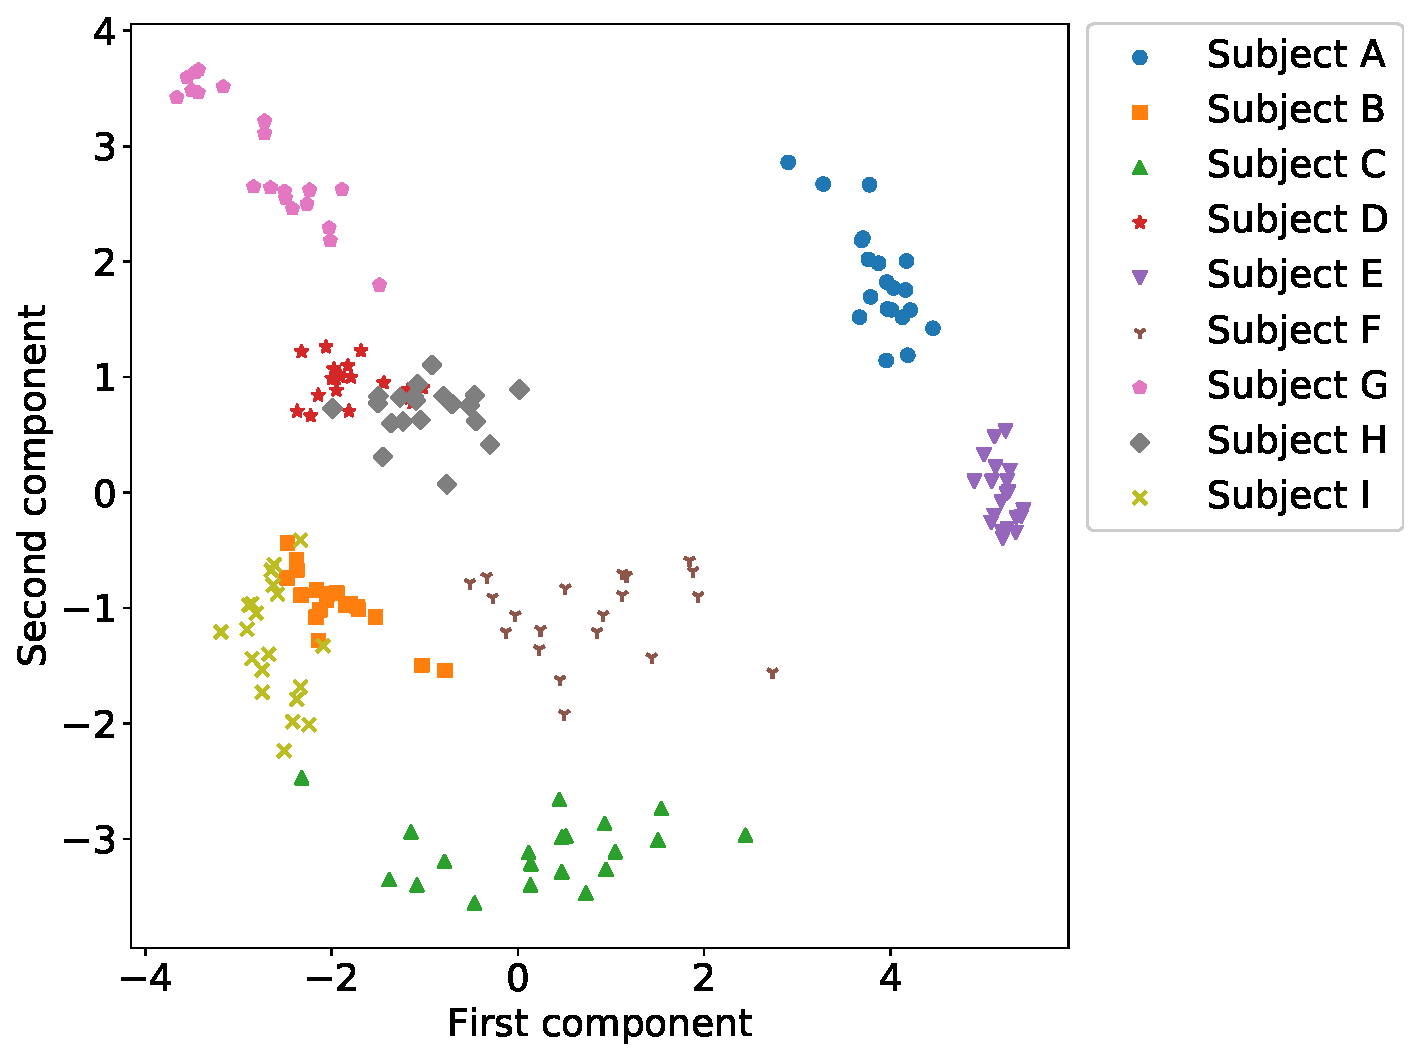
\includegraphics[width=1\linewidth]{figure/PCA.eps}
  \caption{PCAによる分析結果}
  \label{PCA}
\end{figure}

\section{おわりに}
\label{conclude}
本研究では,圧力センサを内部に取り付けたヘルメットを装着することで頭部の形状を計測し,頭部形状の個人差から二輪車の所有者本人を認証する手法を提案し,プロトタイプデバイスの実装とデータ収集および解析プログラムを作成した.プロトタイプデバイスは市販のフルフェイス型ヘルメットを加工し,圧力センサを取り付けた.実験では,プロトタイプデバイスからデータを取得するためにデータ収集プログラムを作成し,頭部形状データとして被験者9人からそれぞれ2秒間のセンサ値を20回分取得した.解析に用いたプログラムはPythonで実装し,登録データと入力データのマハラノビス距離を計算し,本人認証するか拒否するかの閾値を移動させて認証性能を評価した.評価実験の結果,認証の精度の評価指標であるEERが9名中4名が0.012以下,平均0.076という結果が得られた.この結果より,本手法は本人認証手法として有効であると考えられる.今後はさらなるデータの収集を行い,実環境での提案手法の評価を行う.

\bibliography{references}
\bibliographystyle{junsrt}

\end{document}
